
\minisec{Mic-4}
7-stufige Pipeline
\begin{enumerate}
\item Instruction Fetch Unit
\item Dekodiereinheit: Zerlegt Instruktionen in Opcode/Operanden
\item Queueing: Füllt Mikroinstruktionswarteschlange aus ROM-Tabelle(aufeinanderfolgende Mikroinstruktionen)
\item Lesen
\item ALU
\item Schreiben
\item Speicherzugriff
\end{enumerate}

\minisec{Sprungvorhersage}
Behandlung falscher Sprünge: Schreiben nur auf Schattenregistern (=> rückgangigmachen möglich)
\begin{itemize}
\item Einfache Methode: sprünge Rückwärts wahrnehmen, Vorwärts nicht
\item Statische Sprungvorhersage: Compiler gibt empfehlung
\item Dynamische Methode: History-Tabelle (analog Cache): valid, Tag, Entscheidungs-Bits\\
=> Entscheidungs-Bits anhand Endlichem Automaten, z.B. (Wechsel nach 2 Fehlvorhersagen)
\end{itemize}
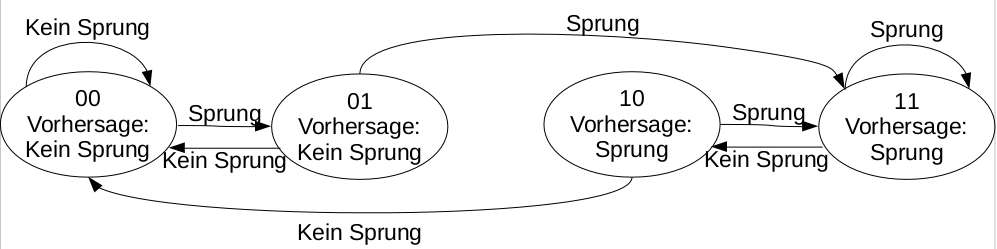
\includegraphics[width=\textwidth]{Sprung}

\minisec{Ausführung außer der Reihe}
Abhängigkeiten: RAW (Read-After-Write) WAW, WAR\\
WAW, WAR => Lösung: Schattenregister\\
Beachten: Änderung der Reihenfolge möglich?

Bsp: (2 Ausführungseinheiten, 1 Zyklus pro Instruktion:)\\
\fbox{
\begin{minipage}{0.5\textwidth}
\begin{enumerate}
\item MUL R1, R2, R1
\item ADD R4, R5, R6
\item SUB R3, R1, R7
\item MUL R8 R3, R3 
\item DIV R11, R4, R4
\item ADD R15, R14, R13
\end{enumerate}
$\Rightarrow$ Abhängigkeiten: RAW: 3-1, 4-3, 5-2 
\end{minipage}} {\Huge $\Rightarrow$}
\fbox{
\begin{minipage}{0.3\textwidth}
Keine Änderung der Reihenfolge:\\
1: 1 2\\
2: 3\\
3: 4 5 \\
4: 6

Änderung der Reihenfolge:\\
1: 1 2\\
2: 3 5 \\
3: 4 6
\end{minipage}
}

Scheduling: (2 Ausführungseinheiten und dekodieren von 2 Instruktionen pro Zyklus)\\
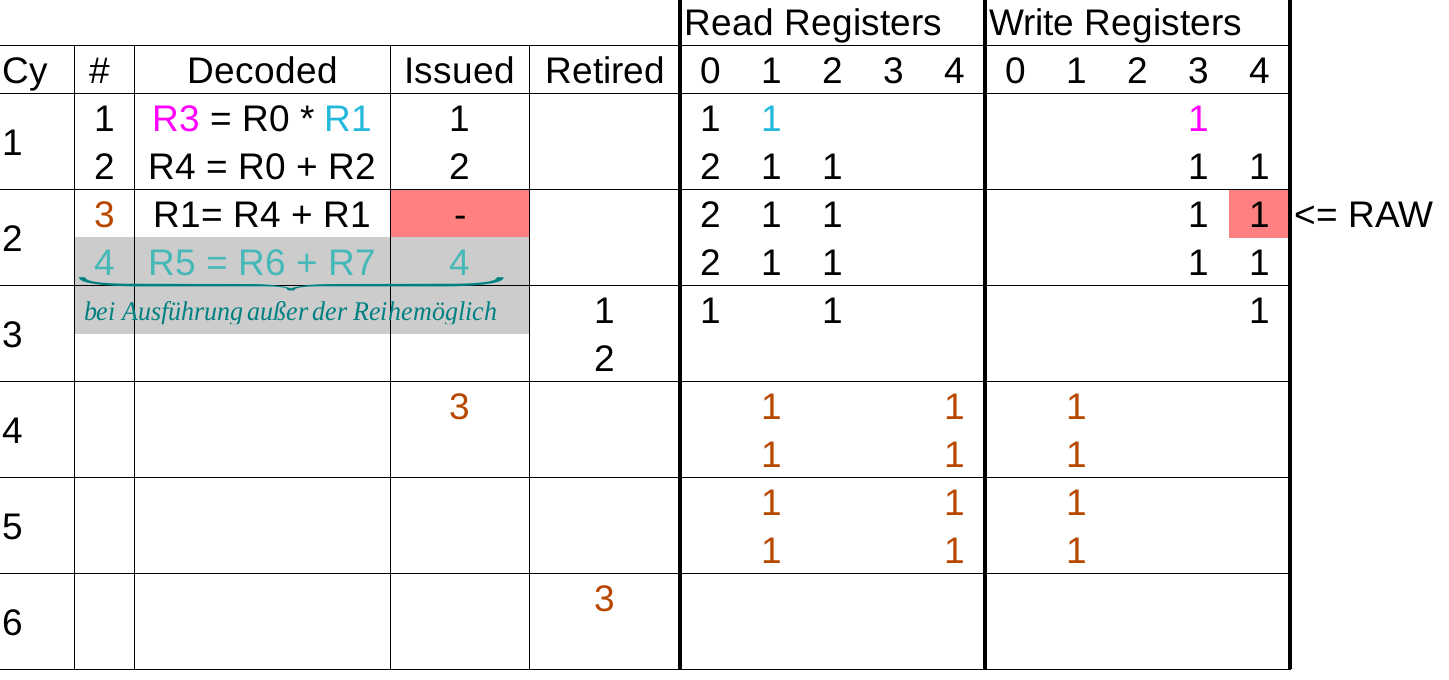
\includegraphics[width=0.7\textwidth]{Sched}

